% Gabarit pandoc des corrigés publiés (brut et guidé). Contenu sans marque ni nom de site.
% Compilation : lualatex (latexmk -lualatex).
% Le Markdown reste la source unique : ne pas éditer ce fichier .tex à la main.
\documentclass[11pt,a4paper]{article}

% --- Moteur, polices (Latin Modern) et langue ---------------------------------
\usepackage{iftex}
\ifLuaTeX\else\errmessage{Ce document se compile avec lualatex}\fi
\usepackage{amsmath,amssymb,mathtools}
\usepackage{fontspec}
% mathrm=sym : \mathrm prend ses glyphes dans la police mathématique (ℓ, μ, Ω), comme KaTeX.
\usepackage[math-style=TeX,bold-style=TeX,mathrm=sym]{unicode-math}
% Repli pour les glyphes absents de Latin Modern (indices et exposants Unicode,
% flèches, filets des schémas en texte, symboles) : DejaVu, puis Latin Modern Math
% (ℓ, lettres mathématiques Unicode des légendes).
\directlua{
  luaotfload.add_fallback("repliTexte", {"DejaVuSerif:mode=harf;", "DejaVuSans:mode=harf;", "file:latinmodern-math.otf:mode=harf;"})
  luaotfload.add_fallback("repliMono", {"DejaVuSansMono:mode=harf;", "DejaVuSans:mode=harf;", "file:latinmodern-math.otf:mode=harf;"})
}
\setmainfont{Latin Modern Roman}[RawFeature={fallback=repliTexte}]
\setsansfont{Latin Modern Sans}[RawFeature={fallback=repliTexte}]
\setmonofont{Latin Modern Mono}[RawFeature={fallback=repliMono}]
\setmathfont{Latin Modern Math}
\usepackage[french]{babel}
\frenchsetup{SmallCapsFigTabCaptions=false}

% --- Mise en page --------------------------------------------------------------
\usepackage[a4paper,margin=2.2cm,headheight=14pt,footskip=1.2cm]{geometry}
\usepackage{microtype}
\setlength{\emergencystretch}{4em}
\tolerance=1500
\setlength{\parindent}{0pt}
\setlength{\parskip}{0.55\baselineskip plus 2pt minus 1pt}
\usepackage{xcolor}
% Gris nommés : babel-french rend « ! » actif dans le document.
\definecolor{gris2}{gray}{0.98}
\definecolor{gris3}{gray}{0.97}
\definecolor{gris5}{gray}{0.95}
\definecolor{gris35}{gray}{0.65}
\definecolor{gris40}{gray}{0.60}
\definecolor{gris45}{gray}{0.55}
\definecolor{gris50}{gray}{0.50}
\definecolor{gris55}{gray}{0.45}
\definecolor{gris60}{gray}{0.40}
\definecolor{gris65}{gray}{0.35}
\definecolor{gris70}{gray}{0.30}
\definecolor{gris80}{gray}{0.20}
\definecolor{gris85}{gray}{0.15}
\usepackage{graphicx}
\usepackage{float}
\usepackage{caption}
\captionsetup{font=small,labelformat=empty,justification=centering}
\usepackage{booktabs,longtable,array,multirow,calc}
\usepackage{siunitx}
\sisetup{locale=FR}
\usepackage[version=4]{mhchem}
\usepackage{listings}
\usepackage{fancyhdr}
\usepackage{lastpage}
\usepackage[most]{tcolorbox}
\usepackage{enumitem}
\setlist{nosep,leftmargin=*,topsep=2pt}
\usepackage[hidelinks,unicode]{hyperref}
\usepackage{bookmark}
\hypersetup{pdftitle={Centrale-Supélec PC — Physique 1 2026},pdfauthor={Rédigé par IA},pdfcreator={LaTeX},pdfsubject={Corrigé guidé}}
\usepackage{xurl}

% --- Pandoc : listes, tableaux, figures ----------------------------------------
\providecommand{\passthrough}[1]{#1}
\providecommand{\tightlist}{\setlength{\itemsep}{0pt}\setlength{\parskip}{0pt}}

\makeatletter
\def\maxwidth{\ifdim\Gin@nat@width>\linewidth\linewidth\else\Gin@nat@width\fi}
\def\maxheight{\ifdim\Gin@nat@height>0.55\textheight 0.55\textheight\else\Gin@nat@height\fi}
\makeatother
\setkeys{Gin}{width=\maxwidth,height=\maxheight,keepaspectratio}
\setcounter{secnumdepth}{-\maxdimen}
\providecommand{\pandocbounded}[1]{#1}
\usepackage{longtable,booktabs,array}

% --- Code (listings) -----------------------------------------------------------
\lstset{
  basicstyle=\ttfamily\small,
  columns=fullflexible,
  keepspaces=true,
  breaklines=true,
  breakatwhitespace=false,
  postbreak=\mbox{\textcolor{gris50}{$\hookrightarrow$}\space},
  frame=single,
  rulecolor=\color{gris35},
  framesep=4pt,
  xleftmargin=5pt,xrightmargin=5pt,
  backgroundcolor=\color{gris3},
  keywordstyle=\bfseries,
  commentstyle=\color{gris65},
  stringstyle=\color{gris80},
  showstringspaces=false,
  tabsize=4,
  extendedchars=true,
  aboveskip=6pt,belowskip=6pt,
}

% --- Macros des corrigés (KaTeX ↔ LaTeX) ---------------------------------------
% Les corrigés sont écrits pour KaTeX : on définit ici ce que KaTeX connaît et
% que LaTeX n'a pas, sans jamais retoucher le Markdown.
\providecommand{\R}{\mathbb{R}}
\providecommand{\N}{\mathbb{N}}
\providecommand{\Z}{\mathbb{Z}}
\providecommand{\Q}{\mathbb{Q}}
\providecommand{\C}{\mathbb{C}}
\providecommand{\dd}{\mathrm{d}}
\providecommand{\llbracket}{\lBrack}
\providecommand{\rrbracket}{\rBrack}
\providecommand{\lBrace}{\lbrace}
\providecommand{\rBrace}{\rbrace}
\providecommand{\Box}{\square}
\providecommand{\Diamond}{\lozenge}
\providecommand{\varnothing}{\emptyset}
\providecommand{\argmax}{\operatorname*{arg\,max}}
\providecommand{\argmin}{\operatorname*{arg\,min}}
\renewcommand{\leq}{\leqslant}
\renewcommand{\geq}{\geqslant}

% Équation hors texte : réduite à la largeur de la ligne si elle déborde.
\newsavebox{\boiteequation}
\newcommand{\equationajustee}[1]{%
  \sbox{\boiteequation}{$\displaystyle #1$}%
  \ifdim\wd\boiteequation>\linewidth
    \[\resizebox{\linewidth}{!}{\usebox{\boiteequation}}\]%
  \else
    \[#1\]%
  \fi}

% --- Encadrés pédagogiques (sobres, lisibles en noir et blanc) -----------------
\tcbset{
  encadre/.style={
    enhanced,breakable,sharp corners,
    colback=white,colframe=gris55,
    boxrule=0.4pt,leftrule=2.2pt,
    left=6pt,right=6pt,top=3pt,bottom=3pt,
    before skip=6pt,after skip=6pt,
    fonttitle=\bfseries\small,coltitle=black,
    attach title to upper,after title={\quad},
    parbox=false,
  }
}
\newtcolorbox{indication}[1]{encadre,colframe=gris45,colback=gris2,title={Indication~#1}}
\newtcolorbox{methode}{encadre,colframe=gris70,title={Méthode}}
\newtcolorbox{piege}{encadre,colframe=gris85,boxrule=0.8pt,leftrule=2.2pt,title={Piège}}
\newtcolorbox{jury}{encadre,colframe=gris60,colback=gris5,title={Jury}}
\newtcolorbox{encadrenote}{encadre,colframe=gris40}

% --- Titres de section ---------------------------------------------------------
\usepackage{titlesec}
\titleformat{\section}{\Large\bfseries}{}{0pt}{}
\titleformat{\subsection}{\large\bfseries}{}{0pt}{}
\titleformat{\subsubsection}{\normalsize\bfseries}{}{0pt}{}
\titlespacing*{\section}{0pt}{14pt plus 4pt minus 2pt}{6pt}
\titlespacing*{\subsection}{0pt}{10pt plus 3pt minus 2pt}{4pt}
\titlespacing*{\subsubsection}{0pt}{8pt plus 2pt minus 2pt}{2pt}

% --- En-tête et pied de page ---------------------------------------------------
\pagestyle{fancy}
\fancyhf{}
\fancyhead[L]{\small\textsc{Corrigé guidé} · Centrale-Supélec PC}
\fancyhead[R]{\small Physique 1 2026}
\fancyfoot[L]{\footnotesize Corrigé rédigé par IA, non officiel}
\fancyfoot[R]{\footnotesize \thepage\,/\,\pageref*{LastPage}}
\renewcommand{\headrulewidth}{0.4pt}
\renewcommand{\footrulewidth}{0pt}
\fancypagestyle{plain}{\fancyhf{}\fancyfoot[R]{\footnotesize \thepage\,/\,\pageref*{LastPage}}\fancyfoot[L]{\footnotesize Corrigé rédigé par IA, non officiel}\renewcommand{\headrulewidth}{0pt}}

\begin{document}
\thispagestyle{plain}
\begin{center}
  {\small\scshape Corrigé guidé}\par\smallskip
  {\LARGE\bfseries Centrale-Supélec PC — Physique 1 2026\par}\medskip
  {\large Centrale-Supélec · PC · Physique 1 · 2026\par}
\end{center}
\vspace{2pt}\hrule\vspace{8pt}

\emph{Corrigé rédigé par IA, non officiel. Signalez toute erreur.}

\hypertarget{pruxe9sentation-du-sujet}{%
\section{Présentation du sujet}\label{pruxe9sentation-du-sujet}}

\textbf{Thème.} « Autour des gouttes et des bulles » : trois phénomènes de physique des interfaces, traités dans trois parties \textbf{totalement indépendantes}. L'épreuve dure 4 heures, avec calculatrice. Elle compte 50 questions : 22 en partie A, 17 en partie B, 11 en partie C.

\begin{itemize}
\tightlist
\item
  \textbf{Partie A --- Évaporation d'une goutte d'eau (Q1 à Q22).} Diffusion de la vapeur autour d'une goutte sphérique en régime quasi stationnaire, conduisant à la loi en \(r^2\) (Q1 à Q9). Couplage avec la thermique : la goutte se refroidit, ce qu'on résout par dichotomie en Python puis par un modèle affine (Q10 à Q18). Correction radiative (Q19, Q20) et application au psychromètre (Q21, Q22).
\item
  \textbf{Partie B --- Spin coating (Q23 à Q39).} Mécanique des fluides visqueux dans un référentiel tournant : on simplifie Navier-Stokes par ordres de grandeur jusqu'à l'équation de lubrification, puis on écrit le profil de vitesse, le débit et un bilan de masse. On aboutit à la loi \(h\propto t^{-1/2}\) de l'épaisseur du film.
\item
  \textbf{Partie C --- Interférométrie sur une bulle (Q40 à Q50).} Montage de collimation, lame à faces parallèles en transmission, ondes multiples (fonction d'Airy), contraste et finesse. On termine par la lecture de photographies réelles et l'ajustement d'une loi \(h(\theta)\) à partir de positions de franges.
\end{itemize}

\textbf{Notions du programme mobilisées.} Corps pur diphasé ; diffusion de particules (loi de Fick, bilans en géométrie sphérique) ; diffusion thermique (loi de Fourier, résistance thermique) ; rayonnement linéarisé ; premier principe pour un système ouvert ; dichotomie en Python ; référentiels non galiléens ; Navier-Stokes, nombre de Reynolds, conditions aux limites ; bilans de masse locaux ; optique géométrique (Snell-Descartes, lentilles) ; interférences (différence de marche, contraste), sommes géométriques complexes ; exploitation de données par linéarisation.

\textbf{Difficulté et longueur.} Le sujet est long mais guidé : beaucoup de résultats intermédiaires sont donnés, ce qui permet de rebondir. Les questions à \textbf{initiative} (numéro souligné) sont \textbf{Q18, Q22 et Q50}. Les plus délicates sont les ordres de grandeur de la partie B (Q24, Q28, Q29), qui demandent de construire soi-même une échelle de vitesse, et Q49, une question ouverte d'interprétation des photographies.

\textbf{À ne pas laisser passer.} Q1 à Q4, Q6 à Q9, Q11, Q12, Q19, Q21 ; Q23, Q26, Q27, Q30 à Q38 ; Q41 à Q48. Ce sont des calculs de cours rapides, souvent avec le résultat donné.

\textbf{Gestion du temps.} Environ 1 h 40 pour A, 1 h 15 pour B, 1 h 05 pour C. Les parties étant indépendantes, on peut commencer par celle qu'on maîtrise le mieux. Il faut garder du temps pour Q50, courte si l'on a bien compris l'identification des ordres de franges.

\hypertarget{partie-a-uxe9vaporation-dune-goutte-deau}{%
\section{Partie A --- Évaporation d'une goutte d'eau}\label{partie-a-uxe9vaporation-dune-goutte-deau}}

On décrit d'abord une goutte isotherme dont la vapeur diffuse vers l'infini (Fick, régime quasi stationnaire, bilan de masse). On couple ensuite cette diffusion à la thermique : la vaporisation refroidit la goutte, ce qui ralentit l'évaporation. Le psychromètre exploite ce refroidissement pour mesurer l'humidité.

\hypertarget{question-1}{%
\subsection{Question 1}\label{question-1}}

\begin{indication}{1}

Question de cours sur le corps pur diphasé : de quel équilibre parle-t-on, et entre quelles phases ?

\end{indication}

\begin{indication}{2}

Pour le sens de variation, pensez à la courbe de vaporisation du diagramme \((T,p)\) ou aux deux valeurs numériques fournies en fin d'énoncé.

\end{indication}

\hypertarget{solution}{%
\subsubsection{Solution}\label{solution}}

À la température \(T\), la pression de vapeur saturante \(p_{\text{sat}}(T)\) d'un corps pur est la pression de la vapeur \textbf{en équilibre avec le liquide}. C'est l'ordonnée, à l'abscisse \(T\), de la courbe de vaporisation du diagramme \((T,p)\). Pour \(p<p_{\text{sat}}(T)\), seule la vapeur est stable ; pour \(p>p_{\text{sat}}(T)\), seul le liquide l'est.

\(p_{\text{sat}}\) est une \textbf{fonction croissante de \(T\)} : elle passe de 0,61 kPa à 273,15 K à 2,3 kPa à 293,15 K (données). La relation de Clausius-Clapeyron (6), donnée plus loin avec \(\Delta h_{\text{vap}}>0\), traduit cette croissance rapide, quasi exponentielle en \(-1/T\).

\begin{piege}

Dire « pression maximale de la vapeur » sans préciser « en équilibre avec le liquide » est insuffisant. Et \(p_{\text{sat}}\) dépend de la seule température, pas de la pression totale.

\end{piege}

\hypertarget{question-2}{%
\subsection{Question 2}\label{question-2}}

\begin{indication}{1}

Cherchez les invariances du problème complet : géométrie, conditions aux limites, milieu extérieur.

\end{indication}

\begin{indication}{2}

Une fois établi que \(c\) ne dépend que de \(r\) et \(t\), la loi de Fick et l'expression du gradient en coordonnées sphériques (formulaire) donnent la direction du courant.

\end{indication}

\hypertarget{solution-1}{%
\subsubsection{Solution}\label{solution-1}}

La pesanteur est négligée, la goutte est une sphère de centre \(O\) et l'air lointain est homogène. L'ensemble du problème est donc invariant par toute rotation autour de \(O\). La concentration, effet de ces causes, possède la même invariance : \(c(\vec r,t)=c(r,t)\) en coordonnées sphériques de centre \(O\).

Le gradient sphérique se réduit alors à \(\dfrac{\partial c}{\partial r}\vec e_r\), et \(\vec\jmath_m=-D\,\dfrac{\partial c}{\partial r}\,\vec e_r\) est radial, de norme fonction de \((r,t)\) seulement : \textbf{le flux est à symétrie sphérique.}

\begin{methode}

Un argument de symétrie porte sur \textbf{tout} le problème (géométrie, conditions aux limites, forces), pas seulement sur la forme de l'objet. C'est l'absence de pesanteur, que l'énoncé précise, qui supprime la direction verticale.

\end{methode}

\hypertarget{question-3}{%
\subsection{Question 3}\label{question-3}}

\begin{indication}{1}

Loi phénoménologique de cours ; les unités se déduisent de celles de \(c\) (concentration en \textbf{masse}).

\end{indication}

\hypertarget{solution-2}{%
\subsubsection{Solution}\label{solution-2}}

\equationajustee{\boxed{\vec\jmath_m=-D\,\overrightarrow{\text{grad}}\,c}}

avec \(c\) en kg·m⁻³, \(\vec\jmath_m\) en kg·m⁻²·s⁻¹ (masse traversant une unité de surface par unité de temps) et \(D\) en m²·s⁻¹. Le signe moins traduit le transport des zones concentrées vers les zones diluées.

\hypertarget{question-4}{%
\subsection{Question 4}\label{question-4}}

\begin{indication}{1}

La vapeur d'eau est un gaz parfait : reliez la masse de vapeur contenue dans un volume \(V\) à sa pression partielle.

\end{indication}

\begin{indication}{2}

À la surface, l'énoncé parle d'équilibre liquide-vapeur ; à l'infini, la définition de \(\mathcal R_H\) fait le reste.

\end{indication}

\hypertarget{solution-3}{%
\subsubsection{Solution}\label{solution-3}}

Pour \(n\) moles de vapeur dans le volume \(V\) sous la pression partielle \(p\), la loi des gaz parfaits et la masse s'écrivent

\equationajustee{\begin{aligned}
pV&=nRT\\
m&=nM_{\text{eau}},
\end{aligned}}

donc

\equationajustee{\boxed{c(r,t)=\frac{M_{\text{eau}}\,p(r,t)}{RT}}}

\begin{itemize}
\tightlist
\item
  En \(r=r_g\), il y a équilibre liquide-vapeur : \(p=p_{\text{sat}}(T)\), d'où \(c(r_g)=c_{\text{sat}}=\dfrac{M_{\text{eau}}p_{\text{sat}}(T)}{RT}\).
\item
  Pour \(r\to\infty\), \(p=p_\infty=\mathcal R_H\,p_{\text{sat}}(T)\), d'où \(c(\infty)=c_\infty=\mathcal R_H\,c_{\text{sat}}\).
\end{itemize}

Comme \(\mathcal R_H\le1\), la concentration décroît de la goutte vers l'infini : la vapeur diffuse vers l'extérieur.

\begin{piege}

La masse molaire de l'air n'intervient pas : \(c\) est la concentration de la \textbf{vapeur d'eau}, qui se calcule avec \(M_{\text{eau}}\) et la pression \textbf{partielle}.

\end{piege}

\hypertarget{question-5}{%
\subsection{Question 5}\label{question-5}}

\begin{indication}{1}

L'approximation compare deux durées : laquelle mesure l'établissement du profil diffusif, laquelle mesure l'évolution de la source ?

\end{indication}

\begin{indication}{2}

L'équation de diffusion associe à une longueur \(L\) un temps en \(L^2/D\). Quelle est la seule longueur du problème ?

\end{indication}

\hypertarget{solution-4}{%
\subsubsection{Solution}\label{solution-4}}

Le profil de concentration s'établit sur l'échelle \(r_g\) en \(\tau_{\text{diff}}\sim r_g^2/D\) ; la goutte évolue sur sa durée de vie \(t_0\). Le critère est

\equationajustee{\boxed{\tau_{\text{diff}}=\frac{r_{g0}^2}{D}\ll t_0}}

\begin{jury}

Un critère \textbf{quantitatif} est demandé : une inégalité entre deux grandeurs explicites, et non une phrase du type « la goutte évolue lentement ».

\end{jury}

\hypertarget{question-6}{%
\subsection{Question 6}\label{question-6}}

\begin{indication}{1}

Le flux étant conservatif, le flux total à travers une sphère de rayon \(r\) ne dépend pas de \(r\). Utilisez-le comme constante.

\end{indication}

\begin{indication}{2}

Exprimez ce flux avec Fick, séparez les variables et intégrez de \(r_g\) à l'infini avec les conditions de Q4.

\end{indication}

\hypertarget{solution-5}{%
\subsubsection{Solution}\label{solution-5}}

À travers la sphère de rayon \(r>r_g\), le flux

\equationajustee{\begin{aligned}
\phi_m&=4\pi r^2j_m\\
&=-4\pi r^2D\,\frac{\mathrm dc}{\mathrm dr}
\end{aligned}}

est indépendant de \(r\). Alors

\equationajustee{\begin{aligned}
\frac{\mathrm dc}{\mathrm dr}&=-\frac{\phi_m}{4\pi Dr^2}\\
c(r)&=c_\infty+\frac{\phi_m}{4\pi Dr}.
\end{aligned}}

La condition \(c(r_g)=c_{\text{sat}}\) donne \(\phi_m=4\pi Dr_g(c_{\text{sat}}-c_\infty)\), soit

\equationajustee{\boxed{\phi_m=4\pi r_g\,\frac{M_{\text{eau}}Dp_{\text{sat}}(T)}{RT}(1-\mathcal R_H)}}

Le profil est en \(1/r\) et le flux est proportionnel à \(r_g\), et non à la surface \(r_g^2\). Le gradient en surface, en \(1/r_g\), compense.

\begin{methode}

En régime stationnaire à symétrie sphérique sans source, écrire « flux total = constante » est plus rapide que de résoudre \(\Delta c=0\). Le même calcul servira pour la thermique en Q12.

\end{methode}

\hypertarget{question-7}{%
\subsection{Question 7}\label{question-7}}

\begin{indication}{1}

Première manière : ce qui sort par la surface pendant \(\mathrm dt\). Seconde manière : la masse d'une sphère de rayon \(r_g\).

\end{indication}

\hypertarget{solution-6}{%
\subsubsection{Solution}\label{solution-6}}

D'une part, \(\mathrm dm=-\phi_m\,\mathrm dt\). D'autre part, \(m=\tfrac43\pi r_g^3\mu_{\text{eau}}\) (liquide incompressible), donc \(\mathrm dm=4\pi r_g^2\mu_{\text{eau}}\,\mathrm dr_g\). En égalant et en simplifiant par \(4\pi r_g\ne0\) :

\equationajustee{\boxed{r_g\frac{\mathrm dr_g}{\mathrm dt}=-\frac{M_{\text{eau}}Dp_{\text{sat}}(T)}{\mu_{\text{eau}}RT}(1-\mathcal R_H)}}

\hypertarget{question-8}{%
\subsection{Question 8}\label{question-8}}

\begin{indication}{1}

Le membre de gauche est la dérivée d'une fonction simple de \(r_g\).

\end{indication}

\hypertarget{solution-7}{%
\subsubsection{Solution}\label{solution-7}}

On pose \(\kappa=\dfrac{M_{\text{eau}}Dp_{\text{sat}}(T)}{\mu_{\text{eau}}RT}(1-\mathcal R_H)\). Alors \(\tfrac12\,\mathrm d(r_g^2)/\mathrm dt=-\kappa\), donc \(r_g^2=r_{g0}^2-2\kappa t\) et

\equationajustee{\boxed{r_g(t)=r_{g0}\sqrt{1-t/t_0}}}

avec

\equationajustee{\boxed{t_0=\frac{\mu_{\text{eau}}RT\,r_{g0}^2}{2M_{\text{eau}}Dp_{\text{sat}}(T)(1-\mathcal R_H)}}}

C'est la « loi en \(d^2\) » : le carré du diamètre décroît linéairement et la goutte disparaît en un temps fini.

\begin{piege}

Ce n'est pas une décroissance exponentielle : l'équation n'est pas linéaire en \(r_g\).

\end{piege}

\hypertarget{question-9}{%
\subsection{Question 9}\label{question-9}}

\begin{indication}{1}

Application numérique directe, toutes grandeurs en unités SI (\(M_{\text{eau}}\) en kg·mol⁻¹, \(T\) en K).

\end{indication}

\begin{indication}{2}

Pour la validité, revenez au critère de Q5 et calculez les deux durées.

\end{indication}

\hypertarget{solution-8}{%
\subsubsection{Solution}\label{solution-8}}

\equationajustee{t_0=\frac{10^3\times8{,}314\times293{,}15\times10^{-6}}{2\times18\times10^{-3}\times2{,}4\times10^{-5}\times2{,}3\times10^3},}

soit

\equationajustee{\boxed{t_0\approx1{,}2\times10^3\ \text{s}\approx20\ \text{min}}}

On a \(\tau_{\text{diff}}=r_{g0}^2/D\), soit \(4{,}2\times10^{-2}\) s, d'où \(\tau_{\text{diff}}/t_0\approx3\times10^{-5}\ll1\) : \textbf{l'approximation est largement valide.}

En effet, \(\tau_{\text{diff}}/t_0=2c_{\text{sat}}(1-\mathcal R_H)/\mu_{\text{eau}}\) : la vapeur saturante est des dizaines de milliers de fois moins dense que le liquide.

\begin{methode}

Toujours confronter un résultat à l'intuition : une goutte millimétrique qui s'évapore en une vingtaine de minutes dans l'air sec est plausible.

\end{methode}

\hypertarget{question-10}{%
\subsection{Question 10}\label{question-10}}

\begin{indication}{1}

Une donnée de l'énoncé ne sert qu'ici : la conductivité thermique de l'eau liquide.

\end{indication}

\begin{indication}{2}

Comparez les résistances thermiques de conduction dans la goutte et dans l'air, qui ont la même géométrie. On peut confirmer par un temps de diffusion thermique dans la goutte.

\end{indication}

\hypertarget{solution-9}{%
\subsubsection{Solution}\label{solution-9}}

À géométrie et échelle égales, les conductances valent environ \(\lambda_{\text{eau}}r_g\) dans la goutte et \(\lambda_{\text{air}}r_g\) dans l'air. Le rapport des chutes de température (nombre de Biot) est \(\lambda_{\text{air}}/\lambda_{\text{eau}}=0{,}026/0{,}61\approx4\times10^{-2}\ll1\) : presque tout l'écart de température se situe dans l'air.

De plus, \(\tau_{\text{th}}=\mu_{\text{eau}}c_{\text{eau}}r_{g0}^2/\lambda_{\text{eau}}\approx7\) s \(\ll t_0\). \textbf{La température de la goutte est uniforme.}

\hypertarget{question-11}{%
\subsection{Question 11}\label{question-11}}

\begin{indication}{1}

Faut-il fournir ou récupérer de l'énergie pour vaporiser un liquide ? D'où vient cette énergie ?

\end{indication}

\hypertarget{solution-10}{%
\subsubsection{Solution}\label{solution-10}}

La vaporisation absorbe \(\Delta h_{\text{vap}}>0\) par kilogramme : elle est \textbf{endothermique}. La goutte se refroidit jusqu'à ce que la chaleur reçue de l'air compense la puissance de vaporisation : \(\boxed{T_g<T_\infty}\).

\hypertarget{question-12}{%
\subsection{Question 12}\label{question-12}}

\begin{indication}{1}

C'est le calcul de Q6, transposé à la diffusion thermique.

\end{indication}

\begin{indication}{2}

Le flux thermique total à travers une sphère de rayon \(r\) est conservatif. Intégrez \(T(r)\) entre \(r_g\) (où \(T=T_g\)) et l'infini.

\end{indication}

\hypertarget{solution-11}{%
\subsubsection{Solution}\label{solution-11}}

Le flux sortant \(\Phi=-4\pi r^2\lambda_{\text{air}}\,\mathrm dT/\mathrm dr\) ne dépend pas de \(r\). Donc \(T(r)=T_\infty+(T_g-T_\infty)\,r_g/r\), et le flux \textbf{reçu} par la goutte vaut

\equationajustee{\phi_{\text{th,d}}=4\pi\lambda_{\text{air}}r_g(T_\infty-T_g),}

d'où

\equationajustee{\boxed{R_{\text{th,d}}=\frac1{4\pi\lambda_{\text{air}}r_g}}}

\(R_{\text{th,d}}\) s'exprime en K·W⁻¹.

\begin{piege}

Ne pas confondre avec une résistance surfacique (K·m²·W⁻¹) : \(R_{\text{th,d}}\) porte sur le flux total.

\end{piege}

\hypertarget{question-13}{%
\subsection{Question 13}\label{question-13}}

\begin{indication}{1}

En régime quasi stationnaire, la température de la goutte ne varie pas : où passe l'énergie reçue de l'air ?

\end{indication}

\begin{indication}{2}

Écrivez l'égalité entre le flux thermique reçu et la puissance de vaporisation \(\Delta h_{\text{vap}}\phi_m\), puis factorisez \(p_{\text{sat}}(T_\infty)/T_\infty\).

\end{indication}

\hypertarget{solution-12}{%
\subsubsection{Solution}\label{solution-12}}

La goutte est à température constante et son énergie interne sensible ne varie pas notablement. La puissance reçue alimente donc entièrement la vaporisation : \(\phi_{\text{th,d}}=\Delta h_{\text{vap}}\phi_m\). Avec Q12 et (4) :

\equationajustee{4\pi\lambda_{\text{air}}r_g(T_\infty-T_g)=\Delta h_{\text{vap}}\,4\pi r_g\frac{M_{\text{eau}}D}{R}\left[\frac{p_{\text{sat}}(T_g)}{T_g}-\frac{p_\infty}{T_\infty}\right].}

On simplifie par \(4\pi r_g\), on factorise \(p_{\text{sat}}(T_\infty)/T_\infty\) et on utilise \(\mathcal R_H=p_\infty/p_{\text{sat}}(T_\infty)\) :

\equationajustee{\boxed{T_\infty-T_g=\frac{\Delta h_{\text{vap}}M_{\text{eau}}Dp_{\text{sat}}(T_\infty)}{\lambda_{\text{air}}RT_\infty}\left(\frac{p_{\text{sat}}(T_g)}{T_g}\frac{T_\infty}{p_{\text{sat}}(T_\infty)}-\mathcal R_H\right)}}

L'écart \textbf{ne dépend pas de \(r_g\)} ; ce point sera décisif en Q18.

\begin{piege}

\(\Delta h_{\text{vap}}\) est \textbf{massique} : il multiplie un flux de masse. Le bilan porte sur la goutte, qui reçoit \(\phi_{\text{th,d}}\) et perd \(\phi_m\).

\end{piege}

\hypertarget{question-14}{%
\subsection{Question 14}\label{question-14}}

\begin{indication}{1}

La dichotomie cherche un zéro : écrivez (5) sous la forme \(f(T_g)=0\) en remplaçant le rapport des pressions par (6), avec les constantes \(C_1\) et \(C_2\) du programme.

\end{indication}

\begin{indication}{2}

Bornes : il faut \(f(a)\) et \(f(b)\) de signes opposés. Utilisez Q11 pour l'une, et l'état liquide de la goutte pour l'autre.

\end{indication}

\hypertarget{solution-13}{%
\subsubsection{Solution}\label{solution-13}}

Avec \(C_1=\dfrac{\Delta h_{\text{vap}}DM_{\text{eau}}p_{\text{sat}}(T_\infty)}{\lambda_{\text{air}}RT_\infty}\) et \(C_2=\dfrac{\Delta h_{\text{vap}}M_{\text{eau}}}R\) :

\begin{lstlisting}[language=Python]
def f(x):
    return Tinf - x - C1*(Tinf/x*np.exp(C2*(1/Tinf - 1/x)) - RH)

a = 273.0   # la goutte reste liquide
b = Tinf    # Tg < Tinf (Q11)
\end{lstlisting}

Les constantes valent \(C_1\approx38\) K et \(C_2\approx5{,}2\times10^3\) K. On a alors

\equationajustee{f(b)=-C_1(1-\mathcal R_H)<0}

et

\equationajustee{f(273)\approx+8{,}8>0 .}

La fonction \(f\) est continue et change de signe, donc \texttt{bisect} converge. Le programme renvoie \(T_g\approx277{,}74\) K à \(10^{-2}\) K près ; une borne \(a=250\) K convient aussi.

\begin{piege}

Trois erreurs typiques : oublier le facteur \(T_\infty/x\) (l'équation (5) porte sur \(p_{\text{sat}}/T\)), inverser \(1/T_\infty-1/x\) dans l'exponentielle, ou proposer des bornes qui n'encadrent pas la racine (\texttt{bisect} lève alors une erreur). Les commentaires du listing comportent deux coquilles sans conséquence : \texttt{Lambda} est une conductivité thermique et \(\Delta h_{\text{vap}}\) s'exprime en J·kg⁻¹.

\end{piege}

\hypertarget{question-15}{%
\subsection{Question 15}\label{question-15}}

\begin{indication}{1}

Le modèle (7) porte sur la \textbf{concentration} saturante, pas sur la pression. Exprimez \(c_{\text{sat}}\) en fonction de \(p_{\text{sat}}\) et \(T\).

\end{indication}

\begin{indication}{2}

Écrivez (7) au point \(T=T_{\text{fus}}\), où \(p_{\text{sat}}\) est connue, et isolez \(\alpha\).

\end{indication}

\hypertarget{solution-14}{%
\subsubsection{Solution}\label{solution-14}}

Avec \(c_{\text{sat}}=M_{\text{eau}}p_{\text{sat}}/(RT)\), l'équation (7) écrite en \(T_{\text{fus}}\) donne

\equationajustee{\boxed{\alpha=\frac1{T_\infty-T_{\text{fus}}}\left[1-\frac{p_{\text{sat}}(T_{\text{fus}})\,T_\infty}{p_{\text{sat}}(T_\infty)\,T_{\text{fus}}}\right]}}

Numériquement, \(\alpha=(1-0{,}265\times1{,}073)/20{,}0\), soit \(\boxed{\alpha\approx3{,}6\times10^{-2}\ \text{K}^{-1}}\).

\begin{piege}

Oublier le facteur \(T_\infty/T_{\text{fus}}\) donne \(3{,}7\times10^{-2}\) K⁻¹ : l'écart numérique est faible, mais la méthode est fausse.

\end{piege}

\hypertarget{question-16}{%
\subsection{Question 16}\label{question-16}}

\begin{indication}{1}

Réécrivez le flux (4) avec des concentrations : il est proportionnel à \(c_{\text{sat}}(T_g)-c_\infty\).

\end{indication}

\begin{indication}{2}

Le bilan d'énergie devient alors linéaire en \(\Delta T\) une fois (7) injecté.

\end{indication}

\hypertarget{solution-15}{%
\subsubsection{Solution}\label{solution-15}}

On a \(\phi_m=4\pi r_gD[c_{\text{sat}}(T_g)-c_\infty]\) et \(c_\infty=\mathcal R_Hc_{\text{sat}}(T_\infty)\). Le bilan d'énergie s'écrit

\equationajustee{\lambda_{\text{air}}\Delta T=\Delta h_{\text{vap}}D\,c_{\text{sat}}(T_\infty)[1-\alpha\Delta T-\mathcal R_H].}

Avec \(K=\Delta h_{\text{vap}}Dc_{\text{sat}}(T_\infty)/\lambda_{\text{air}}\), il donne :

\equationajustee{\boxed{T_\infty-T_g=\frac{K}{1+K\alpha}(1-\mathcal R_H)}}

avec

\equationajustee{\boxed{K=\frac{\Delta h_{\text{vap}}DM_{\text{eau}}p_{\text{sat}}(T_\infty)}{\lambda_{\text{air}}RT_\infty}}}

\(K\) est une température. Pour \(\mathcal R_H=1\), on retrouve bien \(\Delta T=0\).

\hypertarget{question-17}{%
\subsection{Question 17}\label{question-17}}

\begin{indication}{1}

Calculez d'abord \(c_{\text{sat}}(T_\infty)\), puis \(K\) et \(K\alpha\). Pour commenter, comparez à la résolution numérique et au signe attendu de l'erreur du modèle affine.

\end{indication}

\hypertarget{solution-16}{%
\subsubsection{Solution}\label{solution-16}}

\(c_{\text{sat}}(T_\infty)=1{,}70\times10^{-2}\) kg·m⁻³, \(K=37{,}6\) K, \(K\alpha=1{,}35\), d'où

\equationajustee{\boxed{T_\infty-T_g\approx16\ \text{K}}}

C'est proche de l'écart d'environ 15 K donné par la résolution numérique (écart d'environ 5 \%). La fonction \(c_{\text{sat}}(T)\) est convexe et le modèle affine la remplace par une corde, située au-dessus : il surestime \(c_{\text{sat}}(T_g)\), donc l'évaporation et le refroidissement. Le refroidissement est spectaculaire, la goutte est vers 4 °C. On vérifie aussi \(\Delta T/T_\infty\approx5\times10^{-2}\ll1\), ce qui servira en Q19.

\hypertarget{question-18}{%
\subsection{Question 18}\label{question-18}}

\begin{indication}{1}

Reprenez le bilan de masse de Q7 avec le flux (4) : qu'est-ce qui change dans le second membre ? Reste-t-il constant au cours de l'évaporation ?

\end{indication}

\begin{indication}{2}

Le rapport des durées de vie est le rapport des « forces motrices » de l'évaporation, exprimées en concentrations. On peut aussi passer directement par le bilan d'énergie, qui relie \(\phi_m\) à \(\Delta T\).

\end{indication}

\hypertarget{solution-17}{%
\subsubsection{Solution}\label{solution-17}}

Pour \(\mathcal R_H=0\), \(r_g\,\mathrm dr_g/\mathrm dt=-Dc_{\text{sat}}(T_g)/\mu_{\text{eau}}\). D'après Q13, \(T_g\) ne dépend pas de \(r_g\) : le second membre est constant, la loi en \(r^2\) subsiste et

\equationajustee{\begin{aligned}
\frac{t_0'}{t_0}&=\frac{c_{\text{sat}}(T_\infty)}{c_{\text{sat}}(T_g)}\\
&=\frac1{1-\alpha\Delta T}\\
&=\frac1{1-0{,}0358\times16{,}0}\\
&\approx2{,}35 .
\end{aligned}}

De façon équivalente, le bilan d'énergie donne

\equationajustee{\begin{aligned}
\phi_m&=\frac{\phi_{\text{th,d}}}{\Delta h_{\text{vap}}}\\
&=\frac{4\pi\lambda_{\text{air}}r_g\Delta T}{\Delta h_{\text{vap}}},
\end{aligned}}

d'où

\equationajustee{t_0'=\frac{\mu_{\text{eau}}\Delta h_{\text{vap}}r_{g0}^2}{2\lambda_{\text{air}}\Delta T}}

et

\equationajustee{\boxed{t_0'\approx2{,}9\times10^3\ \text{s}\approx48\ \text{min}\approx2{,}3\,t_0}}

Avec \(T_g=277{,}7\) K et la relation (6), on trouve \(c_{\text{sat}}(T_g)/c_{\text{sat}}(T_\infty)=0{,}395\) et \(t_0'\approx3{,}1\times10^3\) s. \textbf{La goutte vit 2,3 à 2,5 fois plus longtemps} que prévu par le modèle isotherme, qui sous-estime donc nettement la durée de vie.

\begin{piege}

Corriger \(t_0\) par le seul rapport \(T_g/T_\infty\approx0{,}95\) ne suffit pas. C'est \(p_{\text{sat}}\), exponentielle en \(-1/T\), qui pilote le flux.

\end{piege}

\begin{jury}

Dans une question à initiative, la démarche est évaluée autant que le résultat. Il faut justifier explicitement que la loi en \(r^2\) reste valable avant de parler d'un nouveau temps d'évaporation.

\end{jury}

\hypertarget{question-19}{%
\subsection{Question 19}\label{question-19}}

\begin{indication}{1}

Développement limité au premier ordre de \(T_g^4=(T_\infty-\Delta T)^4\).

\end{indication}

\hypertarget{solution-18}{%
\subsubsection{Solution}\label{solution-18}}

\(T_\infty^4-T_g^4\approx4T_\infty^3(T_\infty-T_g)\), et \(S_{\text{goutte}}=4\pi r_g^2\), d'où

\equationajustee{\phi_{\text{th,rad}}=16\pi\sigma\varepsilon T_\infty^3r_g^2(T_\infty-T_g),}

d'où

\equationajustee{\boxed{R_{\text{rad}}=\frac1{16\pi\sigma\varepsilon T_\infty^3r_g^2}}}

\hypertarget{question-20}{%
\subsection{Question 20}\label{question-20}}

\begin{indication}{1}

Les deux flux sont proportionnels au même écart de température : comparez les résistances. Lequel des deux flux est le plus grand quand sa résistance est la plus petite ?

\end{indication}

\hypertarget{solution-19}{%
\subsubsection{Solution}\label{solution-19}}

\equationajustee{\begin{aligned}
\frac{\phi_{\text{th,d}}}{\phi_{\text{th,rad}}}&=\frac{R_{\text{rad}}}{R_{\text{th,d}}}\\
&=\frac{\lambda_{\text{air}}}{4\sigma\varepsilon T_\infty^3r_g}.
\end{aligned}}

Ce rapport est grand devant 1 si et seulement si

\equationajustee{\boxed{r_g\ll r_c=\frac{\lambda_{\text{air}}}{4\sigma\varepsilon T_\infty^3}\approx4{,}7\ \text{mm}}}

Pour \(r_{g0}=1\) mm, le rayonnement vaut encore environ 20 \% de la conduction. L'approximation est acceptable sans être excellente, et elle s'améliore quand la goutte rétrécit.

\begin{methode}

\(R_{\text{th,d}}\propto1/r_g\) et \(R_{\text{rad}}\propto1/r_g^2\) : quand deux mécanismes ont des lois d'échelle différentes, une taille critique sépare leurs domaines de prépondérance.

\end{methode}

\hypertarget{question-21}{%
\subsection{Question 21}\label{question-21}}

\begin{indication}{1}

Isolez \(p_\infty(T_\infty)\) dans (9), puis divisez par \(p_{\text{sat}}(T_\infty)\).

\end{indication}

\hypertarget{solution-20}{%
\subsubsection{Solution}\label{solution-20}}

\equationajustee{\boxed{\mathcal R_H=\frac{p_{\text{sat}}(T_g)-\mathcal A\,p_{\text{atm}}(T_\infty-T_g)}{p_{\text{sat}}(T_\infty)}}}

avec \(T_g=T_{\text{hum}}\) et \(T_\infty=T_{\text{sec}}\), les deux grandeurs mesurées. Pour un air saturé, \(\Delta T=0\) et \(\mathcal R_H=1\).

\hypertarget{question-22}{%
\subsection{Question 22}\label{question-22}}

\begin{indication}{1}

Refaites le bilan d'énergie de Q13 avec les flux ventilés (10) et (11). Que deviennent les coefficients de ventilation ?

\end{indication}

\begin{indication}{2}

Pour faire apparaître \(\Delta p\), remplacez les températures des dénominateurs \(p/T\) par une même température moyenne \(\overline T\). L'approximation est justifiée par \(\Delta T\ll T\).

\end{indication}

\hypertarget{solution-21}{%
\subsubsection{Solution}\label{solution-21}}

On a \(f_h\phi_{\text{th,d}}=\Delta h_{\text{vap}}f_{\text{ev}}\phi_m\) avec \(f_h=f_{\text{ev}}\) : on retrouve le bilan de Q13,

\equationajustee{\begin{aligned}
\lambda_{\text{air}}\Delta T&=\frac{\Delta h_{\text{vap}}M_{\text{eau}}D}{R}\left[\frac{p_{\text{sat}}(T_g)}{T_g}-\frac{p_\infty}{T_\infty}\right]\\
&\approx-\frac{\Delta h_{\text{vap}}M_{\text{eau}}D}{R\overline T}\,\Delta p .
\end{aligned}}

Par identification avec (9) :

\equationajustee{\boxed{\mathcal A=\frac{\lambda_{\text{air}}R\overline T}{\Delta h_{\text{vap}}M_{\text{eau}}Dp_{\text{atm}}}}}

Pour \(\overline T\approx285\) K, on obtient \(\mathcal A\approx5{,}9\times10^{-4}\) K⁻¹.

\(\mathcal A\) ne dépend pas de la vitesse \(U\) de ventilation : c'est ce qui rend l'instrument utilisable.

\begin{methode}

L'égalité \(f_{\text{ev}}=f_h\) traduit l'analogie entre transfert de masse et transfert thermique. Dans un rapport de deux flux soumis au même écoulement, les effets de convection se compensent.

\end{methode}

\hypertarget{partie-b-spin-coating}{%
\section{Partie B --- Spin coating}\label{partie-b-spin-coating}}

On simplifie l'équation de Navier-Stokes, écrite dans le référentiel du plateau, par une série d'ordres de grandeur, jusqu'à l'équilibre local entre force centrifuge et viscosité (Q23 à Q30). On en tire le profil de vitesse et le débit (Q31 à Q33), puis un bilan de masse sur une couronne (Q34 à Q36), et enfin la loi d'amincissement d'une goutte modélisée par un cylindre (Q37 à Q39).

\hypertarget{question-23}{%
\subsection{Question 23}\label{question-23}}

\begin{indication}{1}

Nommez chaque terme : deux termes d'accélération, deux forces surfaciques ramenées au volume, et les forces volumiques.

\end{indication}

\begin{indication}{2}

Le référentiel du plateau est en rotation uniforme : quelles forces d'inertie faut-il ajouter au poids ?

\end{indication}

\hypertarget{solution-22}{%
\subsubsection{Solution}\label{solution-22}}

\begin{itemize}
\tightlist
\item
  \(\mu\,\partial\vec v/\partial t\) : accélération locale ;
\item
  \(\mu(\vec v\cdot\overrightarrow{\text{grad}})\vec v\) : accélération convective, non linéaire ; avec le terme précédent, elle forme \(\mu\,\mathrm D\vec v/\mathrm Dt\) ;
\item
  \(-\overrightarrow{\text{grad}}\,p\) : forces de pression par unité de volume ;
\item
  \(\eta\Delta\vec v\) : forces de viscosité par unité de volume (diffusion de quantité de mouvement).
\end{itemize}

Le référentiel tournant à \(\vec\omega=\omega\vec e_z\) constant n'est pas galiléen :

\equationajustee{\boxed{\vec f_{\text{vol}}=\mu\vec g+\mu\omega^2r\,\vec e_r-2\mu\vec\omega\wedge\vec v}}

On y trouve le poids, la force d'inertie d'entraînement (centrifuge, \(r\) = distance à l'axe) et la force de Coriolis. Il n'y a pas de terme en \(\dot{\vec\omega}\) en rotation uniforme.

\begin{piege}

Oublier la force de Coriolis, alors que la question suivante demande précisément de l'évaluer.

\end{piege}

\hypertarget{question-24}{%
\subsection{Question 24}\label{question-24}}

\begin{indication}{1}

Formez le rapport des normes des deux forces : il fait intervenir une vitesse caractéristique que l'énoncé ne donne pas.

\end{indication}

\begin{indication}{2}

Construisez cette vitesse à partir de l'équilibre entre le moteur de l'écoulement (force centrifuge) et son frein (viscosité, avec des gradients sur l'épaisseur \(h\)). Discutez selon la valeur de \(h\).

\end{indication}

\hypertarget{solution-23}{%
\subsubsection{Solution}\label{solution-23}}

On a \(f_{\text{Cor}}/f_{\text{cf}}\sim2v/(\omega r)\). L'équilibre \(\mu\omega^2r\sim\eta v/h^2\) donne \(v\sim\mu\omega^2rh^2/\eta\), d'où

\equationajustee{\frac{f_{\text{Cor}}}{f_{\text{cf}}}\sim\frac{2\omega h^2}{\nu}.}

Les valeurs numériques sont :

\equationajustee{\begin{aligned}
\nu&=\frac{\eta}{\mu}\\
&=3{,}4\times10^{-5}\ \text{m}^2\cdot\text{s}^{-1}\\
\omega&=\frac{2000\times2\pi}{60}\\
&=209\ \text{rad}\cdot\text{s}^{-1}.
\end{aligned}}

Avec la vitesse moyenne dans l'épaisseur, le rapport vaut environ 1 pour \(h_0=0{,}5\) mm. Il tombe à environ \(10^{-2}\) pour \(h=50\) µm. Il ne vaut plus que \(10^{-4}\) pour \(h\approx5\) µm. Le film atteint ces épaisseurs en quelques millisecondes (Q39).

Une estimation plus grossière utilise la vitesse moyenne d'étalement, \((R_{\text{max}}-R_0)/T\approx3\times10^{-3}\) m·s⁻¹. Elle donne \(f_{\text{cf}}/f_{\text{Cor}}\sim3\times10^2\) pour \(r\sim1\) cm. \textbf{Le terme centrifuge est prépondérant} pendant toute la phase qui fixe l'épaisseur finale.

\begin{methode}

Quand l'énoncé ne fournit pas d'échelle de vitesse, on la tire de l'équilibre des forces dominantes, et on le dit. Le même paramètre \(\omega h^2/\nu\) contrôlera aussi Q28 et Q29.

\end{methode}

\begin{jury}

Un ordre de grandeur doit être chiffré et ses hypothèses explicites : dire quelle vitesse on choisit, et pourquoi.

\end{jury}

\hypertarget{question-25}{%
\subsection{Question 25}\label{question-25}}

\begin{indication}{1}

Deux affirmations distinctes : l'indépendance vis-à-vis de \(\theta\) relève de la symétrie, la nullité de \(v_\theta\) relève de l'absence de force orthoradiale.

\end{indication}

\begin{indication}{2}

Coriolis négligée, projetez Navier-Stokes sur \(\vec e_\theta\) : l'équation obtenue a-t-elle un terme source ?

\end{indication}

\hypertarget{solution-24}{%
\subsubsection{Solution}\label{solution-24}}

La goutte, le substrat et les forces restantes (poids, force centrifuge) sont invariants par rotation autour de \((Oz)\). La norme de la vitesse, la pression \(p\) et l'épaisseur \(h\) ne dépendent donc pas de \(\theta\).

Sans force de Coriolis, aucune force n'est orthoradiale et \(\partial p/\partial\theta=0\). La projection sur \(\vec e_\theta\) est une équation homogène en \(v_\theta\). Les conditions aux limites sont \(v_\theta(z=0)=0\) (adhérence au plateau immobile) et \(\partial_zv_\theta(h)=0\).

Le liquide est mis en rotation avec le plateau par diffusion visqueuse en \(h^2/\nu\sim10^{-2}\) s, pendant l'étape d'accélération. Ensuite la solution nulle s'impose : \(\boxed{v_\theta=0}\).

\begin{piege}

« Par symétrie, \(v_\theta=0\) » est faux : une rotation d'ensemble est parfaitement compatible avec la symétrie de révolution. C'est l'absence de force orthoradiale qui annule \(v_\theta\).

\end{piege}

\hypertarget{question-26}{%
\subsection{Question 26}\label{question-26}}

\begin{indication}{1}

Écrivez \(\operatorname{div}\vec v=0\) en cylindriques (formulaire), puis comparez les échelles de variation selon \(r\) et selon \(z\).

\end{indication}

\hypertarget{solution-25}{%
\subsubsection{Solution}\label{solution-25}}

\equationajustee{\frac1r\frac{\partial(rv_r)}{\partial r}+\frac{\partial v_z}{\partial z}=0 .}

Les deux termes sont d'ordres \(v_r/R\) et \(v_z/h\). Ils doivent se compenser, donc \(v_z/v_r\sim h/R\ll1\) :

\equationajustee{\boxed{\vec v\simeq v_r(r,z,t)\,\vec e_r}}

\(v_z\) est petit mais non nul : c'est lui qui fait descendre la surface libre.

\hypertarget{question-27}{%
\subsection{Question 27}\label{question-27}}

\begin{indication}{1}

Passez en revue les cinq termes du laplacien projeté : deux sont rigoureusement nuls d'après Q25.

\end{indication}

\begin{indication}{2}

Pour les autres termes, comparez les échelles de variation de la vitesse radiale : le rayon \(R\) dans la direction radiale, l'épaisseur \(h\) dans la direction verticale.

\end{indication}

\hypertarget{solution-26}{%
\subsubsection{Solution}\label{solution-26}}

Les termes en \(\partial^2v_r/\partial\theta^2\) et \(\partial v_\theta/\partial\theta\) sont nuls. Pour les autres :

\equationajustee{\begin{aligned}
\frac1r\frac{\partial}{\partial r}\Big(r\frac{\partial v_r}{\partial r}\Big)&\sim\frac{v_r}{R^2}\\
\frac{v_r}{r^2}&\sim\frac{v_r}{R^2}\\
\frac{\partial^2v_r}{\partial z^2}&\sim\frac{v_r}{h^2}.
\end{aligned}}

Le dernier domine dans le rapport \((R/h)^2\ge10^2\) :

\equationajustee{\boxed{(\Delta\vec v)\cdot\vec e_r\simeq\frac{\partial^2v_r}{\partial z^2}}}

\hypertarget{question-28}{%
\subsection{Question 28}\label{question-28}}

\begin{indication}{1}

Définissez Re comme le rapport des ordres de grandeur du terme convectif et du terme visqueux.

\end{indication}

\begin{indication}{2}

Dans un film mince, le terme convectif varie sur \(R\) et le terme visqueux sur \(h\) : le rapport pertinent fait apparaître un facteur \(h/R\). Utilisez l'échelle de vitesse de Q24.

\end{indication}

\hypertarget{solution-27}{%
\subsubsection{Solution}\label{solution-27}}

\(\text{Re}=\mu VL/\eta\) compare l'inertie convective à la viscosité. Pour le film, le rapport pertinent est

\equationajustee{\begin{aligned}
\text{Re}^*&=\frac{\mu V^2/R}{\eta V/h^2}\\
&=\frac{\mu Vh}{\eta}\,\frac hR .
\end{aligned}}

Avec \(V\sim\mu\omega^2Rh^2/\eta\), il vaut \(\text{Re}^*\sim(\omega h^2/\nu)^2\) :

\begin{itemize}
\tightlist
\item
  environ 1 au tout début ;
\item
  environ \(10^{-3}\) pour \(h=0{,}1\) mm ;
\item
  environ \(10^{-7}\) pour \(h=10\) µm.
\end{itemize}

Avec la vitesse moyenne d'étalement et \(L=h_0\), on obtient \(\text{Re}\approx5\times10^{-2}\). Hors des premières millisecondes, \(\text{Re}^*\ll1\) : on \textbf{néglige le terme convectif} devant le terme visqueux (écoulement de Stokes).

\begin{piege}

« Re petit donc écoulement laminaire » ne répond pas à la question : ce qui est demandé, c'est quel terme on supprime.

\end{piege}

\hypertarget{question-29}{%
\subsection{Question 29}\label{question-29}}

\begin{indication}{1}

Comparez le temps d'établissement du profil de vitesse dans l'épaisseur (diffusion visqueuse) au temps sur lequel l'épaisseur varie.

\end{indication}

\begin{indication}{2}

Pour ce second temps, utilisez \(h/|\dot h|\) tiré de (14) pour un film uniforme, plutôt que la durée totale du procédé.

\end{indication}

\hypertarget{solution-28}{%
\subsubsection{Solution}\label{solution-28}}

On a \(\tau_\text v\sim h^2/\nu\) et, pour l'épaisseur,

\equationajustee{\begin{aligned}
\tau_h&=\frac{h}{|\dot h|}\\
&=\frac{3\eta}{2\mu\omega^2h^2},
\end{aligned}}

d'où \(\tau_\text v/\tau_h=\tfrac23(\omega h^2/\nu)^2\). Ce rapport vaut :

\begin{itemize}
\tightlist
\item
  environ 1,6 à \(t=0\) ;
\item
  \(3\times10^{-3}\) pour \(h=0{,}1\) mm ;
\item
  \(3\times10^{-7}\) pour \(h=10\) µm.
\end{itemize}

Au-delà de quelques centièmes de seconde, le profil de vitesse suit instantanément l'épaisseur : \textbf{l'écoulement est quasi stationnaire}, et l'on néglige \(\mu\,\partial\vec v/\partial t\). Le bref transitoire initial n'affecte pas l'épaisseur finale, qui oublie \(h_0\) (Q39).

\begin{piege}

Comparer à la période de rotation n'a pas de sens : dans le référentiel tournant, la rotation est stationnaire. Comparer à \(T=30\) s seulement masque le fait que l'épaisseur varie très vite au début.

\end{piege}

\hypertarget{question-30}{%
\subsection{Question 30}\label{question-30}}

\begin{indication}{1}

Récapitulez les termes éliminés aux questions précédentes et par les hypothèses de l'énoncé, puis projetez sur \(\vec e_r\).

\end{indication}

\hypertarget{solution-29}{%
\subsubsection{Solution}\label{solution-29}}

On a éliminé les termes d'inertie (Q28, Q29), le gradient de pression (pression uniforme), le poids (énoncé) et la force de Coriolis (Q24), et \((\Delta\vec v)\cdot\vec e_r\simeq\partial_z^2v_r\) (Q27). Il reste \(0=\mu\omega^2r+\eta\,\partial^2v_r/\partial z^2\) :

\equationajustee{\boxed{\frac{\partial^2v_r}{\partial z^2}=-\frac{\mu\omega^2r}\eta}}

\hypertarget{question-31}{%
\subsection{Question 31}\label{question-31}}

\begin{indication}{1}

En \(z=0\) : paroi solide immobile dans le référentiel d'étude. En \(z=h\) : que vaut la contrainte tangentielle exercée par l'air ?

\end{indication}

\hypertarget{solution-30}{%
\subsubsection{Solution}\label{solution-30}}

En \(z=0\), adhérence : \(\boxed{v_r(r,0,t)=0}\).

En \(z=h\), la contrainte tangentielle est continue ; l'air, environ 2000 fois moins visqueux, n'en exerce pas d'appréciable. Comme la pente de l'interface est faible, la normale est \(\vec e_z\) et cette contrainte s'écrit \(\eta\,\partial v_r/\partial z\), d'où \(\boxed{(\partial v_r/\partial z)_{z=h}=0}\).

\begin{piege}

« La vitesse est maximale en surface » est une conséquence, pas la justification. La justification est l'absence de cisaillement à une surface libre.

\end{piege}

\hypertarget{question-32}{%
\subsection{Question 32}\label{question-32}}

\begin{indication}{1}

Intégrez deux fois en \(z\) à \(r\) et \(t\) fixés. Quelle condition fixe chaque constante ?

\end{indication}

\hypertarget{solution-31}{%
\subsubsection{Solution}\label{solution-31}}

\(\partial_zv_r=-\dfrac{\mu\omega^2r}\eta(z-h)\) (condition en \(h\)), puis, avec la condition en 0 :

\equationajustee{\boxed{v_r=\frac{\mu\omega^2r}{2\eta}\,z(2h-z)}}

Le profil est semi-parabolique, nul à la paroi et maximal à la surface, où il vaut \(\mu\omega^2rh^2/(2\eta)\).

\begin{figure}[H]
\centering
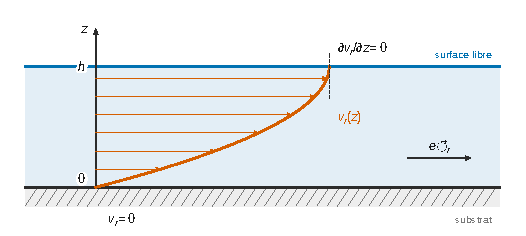
\includegraphics{figures/q32-profil-vitesse-film.pdf}
\caption*{Figure 1 --- Profil de vitesse semi-parabolique dans le film : nul sur
le substrat, maximal et à tangente verticale sur la surface libre}
\end{figure}

\hypertarget{question-33}{%
\subsection{Question 33}\label{question-33}}

\begin{indication}{1}

Intégrez \(v_r\) sur la surface latérale du cylindre de rayon \(r\), d'élément \(r\,\mathrm d\theta\,\mathrm dz\).

\end{indication}

\hypertarget{solution-32}{%
\subsubsection{Solution}\label{solution-32}}

\equationajustee{\begin{aligned}
Q&=2\pi r\int_0^hv_r\,\mathrm dz\\
&=2\pi r\frac{\mu\omega^2r}{\eta}\cdot\frac{h^3}3,
\end{aligned}}

d'où

\equationajustee{\boxed{Q=\frac{2\pi\mu\omega^2r^2}{3\eta}h^3}}

Le débit varie comme \(h^3\) : diviser l'épaisseur par 10 divise le débit par 1000, d'où un amincissement de plus en plus lent.

\hypertarget{question-34}{%
\subsection{Question 34}\label{question-34}}

\begin{indication}{1}

Écrivez la masse de la couronne au premier ordre en \(\mathrm dr\). Faites ensuite varier \(h\) entre \(t\) et \(t+\mathrm dt\).

\end{indication}

\hypertarget{solution-33}{%
\subsubsection{Solution}\label{solution-33}}

\equationajustee{\boxed{\mathrm d^2m=2\pi\mu\,r\,\frac{\partial h}{\partial t}\,\mathrm dr\,\mathrm dt}}

\hypertarget{question-35}{%
\subsection{Question 35}\label{question-35}}

\begin{indication}{1}

Le débit \(Q\) est compté positivement vers l'extérieur : ce qui traverse la face en \(r\) entre dans le système, ce qui traverse la face en \(r+\mathrm dr\) en sort.

\end{indication}

\hypertarget{solution-34}{%
\subsubsection{Solution}\label{solution-34}}

\(\boxed{\delta m_e(r,t)=\mu Q(r,t)\,\mathrm dt}\) et \(\boxed{\delta m_e(r+\mathrm dr,t)=-\mu Q(r+\mathrm dr,t)\,\mathrm dt}\). Rien ne traverse le fond ni la surface libre (le solvant ne s'évapore qu'à l'étape 4). D'où

\equationajustee{\boxed{\delta^2m_e=-\mu\frac{\partial Q}{\partial r}\,\mathrm dr\,\mathrm dt}}

\hypertarget{question-36}{%
\subsection{Question 36}\label{question-36}}

\begin{indication}{1}

Égalez les résultats de Q34 et Q35, puis dérivez le produit \(r^2h^3\) en n'oubliant pas que \(h\) dépend de \(r\).

\end{indication}

\hypertarget{solution-35}{%
\subsubsection{Solution}\label{solution-35}}

\(2\pi r\,\partial_th=-\partial_rQ\), avec \(\partial_r(r^2h^3)=2rh^3+3r^2h^2\partial_rh\). En divisant par \(2\pi r\) :

\equationajustee{\boxed{\frac{\partial h}{\partial t}=-\frac{\mu\omega^2}\eta\left[\frac23h^3+rh^2\frac{\partial h}{\partial r}\right]}}

\begin{methode}

Bilan sur un système ouvert élémentaire : variation de masse = masse entrante. Ce schéma vaut pour toute équation de conservation 1D, en coordonnées cartésiennes, cylindriques ou sphériques.

\end{methode}

\hypertarget{question-37}{%
\subsection{Question 37}\label{question-37}}

\begin{indication}{1}

Dans le modèle cylindrique, que vaut \(\partial h/\partial r\) ? L'équation devient une équation différentielle ordinaire à variables séparables.

\end{indication}

\begin{indication}{2}

Intégrez \(\mathrm dh/h^3\) : la quantité naturelle est \(1/h^2\).

\end{indication}

\hypertarget{solution-36}{%
\subsubsection{Solution}\label{solution-36}}

\(\dfrac{\mathrm dh}{\mathrm dt}=-\dfrac{2\mu\omega^2}{3\eta}h^3\), donc \(\dfrac1{h^2}=\dfrac1{h_0^2}+\dfrac{4\mu\omega^2}{3\eta}t\) :

\equationajustee{\boxed{h(t)=\frac{h_0}{\sqrt{1+t/\tau}}}}

avec

\equationajustee{\boxed{\tau=\frac{3\eta}{4\mu\omega^2h_0^2}}}

Aux temps longs, \(h\approx\sqrt{3\eta/(4\mu\omega^2t)}\) ne dépend plus de \(h_0\).

\begin{piege}

L'équation est non linéaire : une solution exponentielle est fausse.

\end{piege}

\hypertarget{question-38}{%
\subsection{Question 38}\label{question-38}}

\begin{indication}{1}

Que conserve-t-on pendant l'étalement d'un liquide incompressible qui ne s'évapore pas encore ?

\end{indication}

\hypertarget{solution-37}{%
\subsubsection{Solution}\label{solution-37}}

Le volume \(\pi r^2h=\pi R_0^2h_0\) est conservé, d'où \(\boxed{r(t)=R_0(1+t/\tau)^{1/4}}\) : l'étalement latéral est très lent.

\hypertarget{question-39}{%
\subsection{Question 39}\label{question-39}}

\begin{indication}{1}

Convertissez \(\omega\) en rad·s⁻¹. Comparez \(T\) à \(\tau\) avant de simplifier, et contrôlez que la goutte ne déborde pas du substrat.

\end{indication}

\hypertarget{solution-38}{%
\subsubsection{Solution}\label{solution-38}}

\(\omega=209{,}4\) rad·s⁻¹ et

\equationajustee{\tau=\frac{3\times3{,}6\times10^{-2}}{4\times1{,}06\times10^3\times209{,}4^2\times(5\times10^{-4})^2},}

soit

\equationajustee{\boxed{\tau\approx2{,}3\ \text{ms}}}

Comme \(T/\tau\approx1{,}3\times10^4\), \(h(T)\approx h_0\sqrt{\tau/T}\), soit \(\boxed{h(T)\approx4{,}4\ \mu\text{m}}\).

Contrôles : \(r(T)\approx5{,}3\) cm \(<R_{\text{max}}=10\) cm, et l'épaisseur obtenue appartient bien à la gamme annoncée par l'énoncé (d'une dizaine de nanomètres à plusieurs micromètres).

\begin{piege}

Oublier le facteur \(2\pi\) de la conversion tr/min → rad/s change \(\tau\) d'un facteur 40. Le rayon \(R_{\text{max}}\) est fourni pour le contrôle final : une donnée inutilisée doit alerter.

\end{piege}

\hypertarget{partie-c-mesure-de-luxe9paisseur-dune-bulle-par-interfuxe9romuxe9trie}{%
\section{Partie C --- Mesure de l'épaisseur d'une bulle par interférométrie}\label{partie-c-mesure-de-luxe9paisseur-dune-bulle-par-interfuxe9romuxe9trie}}

Le film de la bulle est modélisé localement par une lame à faces parallèles éclairée sous une incidence fixe. On construit la fonction de transmission à ondes multiples (Q42 à Q44), on en tire la position, le contraste et la largeur des franges (Q45 à Q48), puis on interprète les photographies et on ajuste une loi d'épaisseur (Q49, Q50). Les interférences à ondes multiples ne sont pas au programme en tant que telles, mais l'énoncé les construit pas à pas : il suffit de savoir sommer une série géométrique et calculer une différence de marche.

\hypertarget{question-40}{%
\subsection{Question 40}\label{question-40}}

\begin{indication}{1}

Un faisceau parallèle est issu d'un point objet situé au foyer d'une lentille convergente. Quel est le rôle du diaphragme face à une source étendue ?

\end{indication}

\begin{indication}{2}

Pensez à un condenseur pour envoyer un maximum de lumière à travers le diaphragme.

\end{indication}

\hypertarget{solution-39}{%
\subsubsection{Solution}\label{solution-39}}

\begin{enumerate}
\def\labelenumi{\arabic{enumi}.}
\tightlist
\item
  Une lentille condenseur \(L_1\) forme l'image de la lampe au sodium sur un petit diaphragme.
\item
  Le diaphragme constitue une source quasi ponctuelle \(S\).
\item
  \(S\) est placée au foyer objet d'une lentille collimatrice \(L_2\) de grande focale \(f_2'\) : le faisceau émergent est parallèle. La divergence résiduelle vaut environ \(d/f_2'\), où \(d\) est le diamètre du trou.
\end{enumerate}

\begin{figure}[H]
\centering
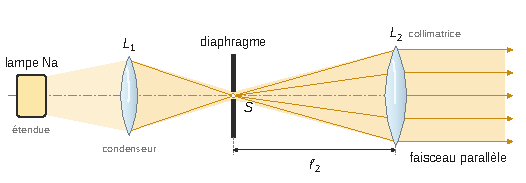
\includegraphics{figures/q40-montage-collimation.pdf}
\caption*{Figure 2 --- Montage de collimation : le condenseur L₁ concentre la
lampe sur le diaphragme, source quasi ponctuelle S placée au foyer objet
de L₂}
\end{figure}

Réglage : la tache lumineuse doit garder le même diamètre quand on éloigne l'écran.

\begin{piege}

Sans diaphragme, chaque point de la source étendue donne un faisceau parallèle de direction différente : le faisceau global diverge et l'angle d'incidence \(\alpha\), sur lequel repose toute la mesure, n'est plus défini.

\end{piege}

\hypertarget{question-41}{%
\subsection{Question 41}\label{question-41}}

\begin{indication}{1}

Loi de Snell-Descartes à l'entrée. Peut-il y avoir réflexion totale quand on passe de l'air à l'huile ?

\end{indication}

\begin{indication}{2}

À la sortie, la normale est la même qu'à l'entrée (faces parallèles).

\end{indication}

\hypertarget{solution-40}{%
\subsubsection{Solution}\label{solution-40}}

La loi de Snell-Descartes à l'entrée donne

\equationajustee{\begin{aligned}
\sin\beta&=\frac{\sin\alpha}{n}\\
&=\frac{0{,}995}{1{,}4}\\
&=0{,}711,
\end{aligned}}

d'où \(\boxed{\beta\approx45{,}3^\circ}\). La lumière pénètre \textbf{toujours} dans le film : on va vers un milieu plus réfringent et \(\sin\alpha/n<1\).

À la sortie, \(n\sin\beta=\sin\alpha'\), donc \(\boxed{\alpha'=\alpha=84{,}2^\circ}\) : les rayons émergents sont parallèles au rayon incident. L'impossibilité de mesurer en incidence rasante vient de ce que \(R\to1\) quand \(\alpha\to90^\circ\) (figure 13), non d'une réflexion totale.

\begin{piege}

La réflexion totale n'existe que du milieu le plus réfringent vers le moins réfringent ; et, par retour inverse de la lumière, un rayon entré dans la lame peut toujours en ressortir.

\end{piege}

\hypertarget{question-42}{%
\subsection{Question 42}\label{question-42}}

\begin{indication}{1}

Le rayon \(k+1\) fait un aller-retour de plus dans la lame. Mais il faut comparer les deux rayons sur un même plan d'onde, perpendiculaire aux rayons émergents.

\end{indication}

\begin{indication}{2}

Le décalage latéral entre deux points d'émergence vaut \(2h\tan\beta\) ; projetez-le sur la direction de propagation dans l'air, puis utilisez Snell-Descartes.

\end{indication}

\hypertarget{solution-41}{%
\subsubsection{Solution}\label{solution-41}}

Le chemin optique supplémentaire dans la lame vaut \(2nh/\cos\beta\). Le rayon \(k\) parcourt en plus dans l'air \(2h\tan\beta\sin\alpha\). Avec \(\sin\alpha=n\sin\beta\) :

\equationajustee{\begin{aligned}
\delta&=\frac{2nh}{\cos\beta}-\frac{2nh\sin^2\beta}{\cos\beta}\\
&=2nh\cos\beta,
\end{aligned}}

d'où

\equationajustee{\boxed{\varphi=\frac{4\pi nh\cos\beta}\lambda}}

Les deux réflexions supplémentaires ont lieu sur des interfaces identiques : il n'y a pas de déphasage additionnel.

\begin{figure}[H]
\centering
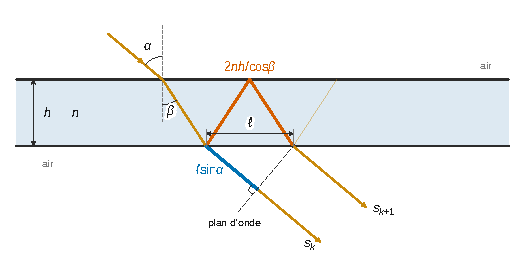
\includegraphics{figures/q42-lame-difference-de-marche.pdf}
\caption*{Figure 3 --- Différence de marche entre deux rayons émergents successifs
: aller-retour supplémentaire 2nh/cos β dans la lame, moins ℓ sin α dans
l'air (angles non à l'échelle)}
\end{figure}

\begin{piege}

Oublier le terme de décalage latéral donne \(2nh/\cos\beta\), faux ici d'un facteur 2.

\end{piege}

\hypertarget{question-43}{%
\subsection{Question 43}\label{question-43}}

\begin{indication}{1}

Que deviennent l'amplitude et la phase d'un rayon à chaque aller-retour supplémentaire ? Vous obtenez une suite géométrique.

\end{indication}

\begin{indication}{2}

Avant de sommer, vérifiez la condition de convergence de la série.

\end{indication}

\hypertarget{solution-42}{%
\subsubsection{Solution}\label{solution-42}}

À chaque aller-retour, l'amplitude est multipliée par \(r^2\) (deux réflexions) et la phase retardée de \(\varphi\) :

\equationajustee{\boxed{\underline s_k=\underline s_1(r^2e^{-i\varphi})^{k-1}}}

Comme \(|r^2e^{-i\varphi}|=r^2<1\), la série converge, et tous les rayons ont le même facteur \(e^{i\omega t}\) :

\equationajustee{\boxed{\underline s=\frac{\underline s_1}{1-r^2e^{-i\varphi}}}}

\hypertarget{question-44}{%
\subsection{Question 44}\label{question-44}}

\begin{indication}{1}

Calculez le module carré du dénominateur et faites apparaître \(\sin^2(\varphi/2)\) grâce au formulaire.

\end{indication}

\begin{indication}{2}

Le numérateur doit être l'intensité \textbf{incidente} : combien de transmissions le rayon 1 a-t-il subies ? Utilisez \(r^2+t^2=1\).

\end{indication}

\hypertarget{solution-43}{%
\subsubsection{Solution}\label{solution-43}}

Le module carré du dénominateur vaut

\equationajustee{|1-r^2e^{-i\varphi}|^2=(1-r^2)^2+4r^2\sin^2(\varphi/2).}

Par ailleurs \(\underline s_1=t^2s_0\), donc \(|\underline s_1|^2=(1-r^2)^2\mathcal I_0\). D'où

\equationajustee{\mathcal I=\frac{\mathcal I_0}{1+m\sin^2(\varphi/2)},}

avec

\equationajustee{\boxed{m=\frac{4r^2}{(1-r^2)^2}}}

\begin{piege}

Laisser \(|\underline s_1|^2\) au numérateur ne démontre pas la formule demandée : c'est \(\mathcal I_0\) qui doit apparaître.

\end{piege}

\hypertarget{question-45}{%
\subsection{Question 45}\label{question-45}}

\begin{indication}{1}

Quand le dénominateur de (16) est-il minimal ? Que vaut alors \(\mathcal I\), et que dire de la lumière réfléchie ?

\end{indication}

\hypertarget{solution-44}{%
\subsubsection{Solution}\label{solution-44}}

\equationajustee{\boxed{\varphi=2p\pi\ (p\in\mathbb Z)}}

Le maximum vaut alors

\equationajustee{\boxed{\mathcal I_{\text{max}}=\mathcal I_0}}

À la résonance, la lame transmet toute la lumière, quel que soit \(r\) : elle n'absorbe pas, et les ondes réfléchies interfèrent destructivement. Les maxima sont périodiques en \(\varphi\). Entre deux maxima, l'intensité tombe à \(\mathcal I_0/(1+m)=\mathcal I_0/12\) pour \(m=11\) : les pics sont fins et contrastés, comme sur la figure 11.

\hypertarget{question-46}{%
\subsection{Question 46}\label{question-46}}

\begin{indication}{1}

Combinez la condition de Q45 avec l'expression de \(\varphi\) de Q42 ; l'écart entre deux ordres successifs donne \(\Delta h\).

\end{indication}

\hypertarget{solution-45}{%
\subsubsection{Solution}\label{solution-45}}

\equationajustee{\boxed{h_p=\frac{p\lambda}{2n\cos\beta}\ (p\in\mathbb N)}}

L'écart d'épaisseur entre deux franges brillantes vaut

\equationajustee{\boxed{\Delta h=\frac{\lambda}{2n\cos\beta}}}

Numériquement :

\equationajustee{\Delta h=\frac{589{,}3\ \text{nm}}{2\times1{,}4\times0{,}704}\approx0{,}30\ \mu\text{m}.}

Ce sont des franges d'égale épaisseur. Ici \(2n\cos\beta\approx1{,}97\) : \(\Delta h\) vaut presque \(\lambda/2\).

\hypertarget{question-47}{%
\subsection{Question 47}\label{question-47}}

\begin{indication}{1}

Définition usuelle du contraste à partir de \(\mathcal I_{\text{max}}\) et \(\mathcal I_{\text{min}}\) ; cherchez \(\mathcal I_{\text{min}}\) dans (16).

\end{indication}

\hypertarget{solution-46}{%
\subsubsection{Solution}\label{solution-46}}

\(\mathcal C=\dfrac{\mathcal I_{\text{max}}-\mathcal I_{\text{min}}}{\mathcal I_{\text{max}}+\mathcal I_{\text{min}}}\), avec \(\mathcal I_{\text{min}}=\mathcal I_0/(1+m)\), d'où \(\mathcal C=\dfrac m{m+2}\) et

\equationajustee{\boxed{\mathcal C=\frac{2r^2}{1+r^4}}}

On obtient \(\mathcal C\approx0{,}85\) pour \(R=r^2\approx0{,}55\) (bord de la bulle). À l'inverse, \(\mathcal C\approx0{,}06\) pour \(R\approx0{,}03\) (incidence normale).

\hypertarget{question-48}{%
\subsection{Question 48}\label{question-48}}

\begin{indication}{1}

Résolvez \(m\sin^2(\varphi/2)=1\) ; l'hypothèse \(m\gg1\) autorise un développement de \(\sin\) près de 0.

\end{indication}

\hypertarget{solution-47}{%
\subsubsection{Solution}\label{solution-47}}

\(\sin(\varphi/2)=\pm1/\sqrt m\), d'où, pour \(m\gg1\) :

\equationajustee{\boxed{\varphi_\pm\approx\pm\frac2{\sqrt m}}}

d'où la largeur à mi-hauteur

\equationajustee{\boxed{\Delta\varphi_{1/2}\approx\frac4{\sqrt m}}}

Pour \(m=11\), \(\Delta\varphi_{1/2}\approx1{,}2\) rad, soit environ 19 \% de l'intervalle entre deux pics. Plus la réflectivité est grande, plus les franges sont fines : c'est le principe du Fabry-Pérot.

\begin{piege}

La largeur à mi-hauteur est \(\varphi_+-\varphi_-\), pas \(\varphi_+\) seul.

\end{piege}

\hypertarget{question-49}{%
\subsection{Question 49}\label{question-49}}

\begin{indication}{1}

Reliez chaque point de l'image à l'angle d'incidence sur la paroi : un rayon passant à la distance \(d\) du centre du disque arrive sous \(\sin\alpha=d/r_0\). Lisez ensuite \(R(\alpha)\) sur la figure 13 et déduisez-en \(m\) et \(\mathcal C\).

\end{indication}

\begin{indication}{2}

Les franges sont d'égale épaisseur : si \(h\) ne dépend que de \(\theta\), quelle est leur forme ? Comment bougent-elles si le haut s'amincit ?

\end{indication}

\begin{indication}{3}

Pour le protocole, le comptage de franges ne donne que des différences d'épaisseur : quel événement observable fixe l'ordre absolu ?

\end{indication}

\hypertarget{solution-48}{%
\subsubsection{Solution}\label{solution-48}}

\emph{Position.} Pour un rayon passant à la distance \(d\) du centre, \(\sin\alpha=d/r_0\). La figure 13 donne :

\begin{longtable}[]{@{}llllll@{}}
\toprule\noalign{}
α & 0° & 60° & 75° & 84,2° & → 90° \\
\midrule\noalign{}
\endhead
\bottomrule\noalign{}
\endlastfoot
\(d/r_0\) & 0 & 0,87 & 0,97 & 0,995 & 1 \\
\(R\) & 0,03 & 0,07 & 0,23 & 0,55 & 1 \\
\(m\) & 0,13 & 0,33 & 1,5 & 11 & \(\to\infty\) \\
\(\mathcal C\) & 0,06 & 0,14 & 0,44 & 0,85 & 1 \\
\end{longtable}

Les franges ne sont contrastées que pour \(\alpha\gtrsim75^\circ\) : elles forment une \textbf{fine couronne sur le pourtour} de la bulle, et l'intérieur paraît uniforme. Tout au bord, \(R\to1\) et rien n'est transmis : le contour est sombre. L'arc à \(0{,}995\,r_0\) concilie fort contraste et transmission mesurable.

\emph{Aspect.} Les franges sont fines (\(\Delta\varphi_{1/2}\approx1{,}2\) rad) et contrastées. Ce sont des franges d'égale épaisseur ; comme \(h\) ne dépend que de \(\theta\), elles suivent les parallèles, vus comme des \textbf{traits horizontaux}. Elles se resserrent vers la base, où \(h\) croît vite : 28,4° entre les franges 1 et 2, 1,1° entre les franges 8 et 9.

\emph{Évolution.} Chaque frange correspond à une épaisseur fixée \(p\Delta h\). Le drainage amincit le haut, donc chaque frange \textbf{descend} : c'est le cas de la ligne tiretée entre \(t=0\) et \(t=370\) s.

Une nouvelle frange naît au sommet chaque fois que \(h(0)\) franchit un multiple de \(\Delta h\). La dernière, apparue à \(t=220\) s (ligne pointillée), est d'ordre \(p=1\) : \(h(0)=\Delta h\approx0{,}30\) µm. Ensuite il n'y a plus de frange au sommet.

D'après (16), quand \(h\to0\), \(\varphi\to0\) et la transmission tend vers \(\mathcal I_0\). Le minimum se situe vers \(h\approx\Delta h/2\). Le « film noir » désigne classiquement, en réflexion, un film de quelques dizaines de nanomètres au plus, qui ne réfléchit presque rien. Son apparition au sommet annonce l'éclatement.

\emph{Protocole.}

\begin{enumerate}
\def\labelenumi{\arabic{enumi}.}
\tightlist
\item
  Filmer à cadence régulière.
\item
  Sur chaque image, relever l'intensité le long de l'arc de rayon \(0{,}995\,r_0\). L'incidence y est uniforme (\(\alpha=84{,}2^\circ\)), donc \(\Delta h\) aussi, et l'angle polaire repère \(\theta\).
\item
  Repérer les maxima \(\theta_k\).
\item
  Fixer les ordres : à l'apparition de la dernière frange au sommet, celle-ci est d'ordre 1, et les suivantes vers le bas sont d'ordre \(2,3,\dots\), d'où \(h(\theta_k)=k\Delta h\). On peut aussi remonter le temps depuis l'éclatement (\(h\to0\)).
\item
  Suivre chaque frange d'image en image (son ordre est conservé) pour obtenir \(h(\theta,t)\), puis interpoler entre les franges.
\end{enumerate}

\begin{piege}

En transmission, un film quasi nul correspond à \(\varphi\approx0\), donc à un \textbf{maximum} de transmission. Prédire un sommet sombre pour un film de quelques nanomètres contredit la formule (16) qu'on vient d'établir.

\end{piege}

\begin{jury}

« Expliquer précisément » appelle des arguments chiffrés tirés des figures (valeurs de \(R\), de \(m\), du contraste), pas seulement une description qualitative.

\end{jury}

\hypertarget{question-50}{%
\subsection{Question 50}\label{question-50}}

\begin{indication}{1}

D'après Q46, le numéro d'une frange donne son épaisseur à une constante près. La phrase « la dernière frange brillante apparaît au sommet » fixe cette constante.

\end{indication}

\begin{indication}{2}

Une loi en \(\cos^{-\ell}\theta\) se teste par passage au logarithme : quelles grandeurs porter en abscisse et en ordonnée pour obtenir une droite passant par l'origine ?

\end{indication}

\hypertarget{solution-49}{%
\subsubsection{Solution}\label{solution-49}}

À \(t=220\) s, la frange 1 du sommet est d'ordre 1 (dernière frange avant \(h\to0\)). La frange \(k\) est d'ordre \(k\), donc \(h_k=k\Delta h\).

Au sommet, \(h_0=\Delta h\), soit \(h_k/h_0=k\). La loi (17) équivaut à

\equationajustee{\ln k=\ell\,\big[-\ln\cos\theta_k\big].}

\begin{longtable}[]{@{}
  >{\raggedright\arraybackslash}p{(\columnwidth - 16\tabcolsep) * \real{0.1111}}
  >{\raggedright\arraybackslash}p{(\columnwidth - 16\tabcolsep) * \real{0.1111}}
  >{\raggedright\arraybackslash}p{(\columnwidth - 16\tabcolsep) * \real{0.1111}}
  >{\raggedright\arraybackslash}p{(\columnwidth - 16\tabcolsep) * \real{0.1111}}
  >{\raggedright\arraybackslash}p{(\columnwidth - 16\tabcolsep) * \real{0.1111}}
  >{\raggedright\arraybackslash}p{(\columnwidth - 16\tabcolsep) * \real{0.1111}}
  >{\raggedright\arraybackslash}p{(\columnwidth - 16\tabcolsep) * \real{0.1111}}
  >{\raggedright\arraybackslash}p{(\columnwidth - 16\tabcolsep) * \real{0.1111}}
  >{\raggedright\arraybackslash}p{(\columnwidth - 16\tabcolsep) * \real{0.1111}}@{}}
\toprule\noalign{}
\begin{minipage}[b]{\linewidth}\raggedright
\(k\)
\end{minipage} & \begin{minipage}[b]{\linewidth}\raggedright
2
\end{minipage} & \begin{minipage}[b]{\linewidth}\raggedright
3
\end{minipage} & \begin{minipage}[b]{\linewidth}\raggedright
4
\end{minipage} & \begin{minipage}[b]{\linewidth}\raggedright
5
\end{minipage} & \begin{minipage}[b]{\linewidth}\raggedright
6
\end{minipage} & \begin{minipage}[b]{\linewidth}\raggedright
7
\end{minipage} & \begin{minipage}[b]{\linewidth}\raggedright
8
\end{minipage} & \begin{minipage}[b]{\linewidth}\raggedright
9
\end{minipage} \\
\midrule\noalign{}
\endhead
\bottomrule\noalign{}
\endlastfoot
\(x_k=-\ln\cos\theta_k\) & 0,128 & 0,202 & 0,256 & 0,297 & 0,331 & 0,361 & 0,386 & 0,408 \\
\(y_k=\ln k\) & 0,693 & 1,099 & 1,386 & 1,609 & 1,792 & 1,946 & 2,079 & 2,197 \\
\(y_k/x_k\) & 5,41 & 5,44 & 5,41 & 5,42 & 5,41 & 5,39 & 5,38 & 5,39 \\
\end{longtable}

Les points, y compris \((0,0)\) pour \(k=1\), sont alignés sur une droite passant par l'origine. La régression libre donne une ordonnée à l'origine de 0,004, et les rapports \(y_k/x_k\) sont constants à 0,6 \% près. La loi (17) est validée, avec

\equationajustee{\boxed{\ell=\frac{\sum x_ky_k}{\sum x_k^2}\approx5{,}4}}

soit

\equationajustee{h(\theta)\approx0{,}30\ \mu\text{m}\times\cos^{-5{,}4}\theta .}

\begin{figure}[H]
\centering
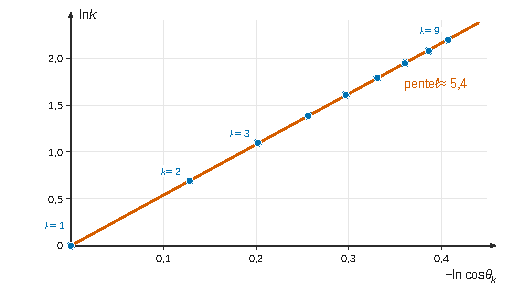
\includegraphics{figures/q50-linearisation-franges.pdf}
\caption*{Figure 4 --- Linéarisation du tableau 1 : ln k en fonction de −ln cos
θₖ, droite passant par l'origine de pente ℓ ≈ 5,4}
\end{figure}

Avec un décalage d'ordre, \(h_k=(k+1)\Delta h\), l'ajustement serait nettement moins bon (ordonnée à l'origine 0,6), ce qui confirme l'identification. L'épaisseur passe de 0,30 µm au sommet à environ 2,7 µm vers 48° : le drainage est très inhomogène.

\begin{methode}

Pour tester une loi de puissance \(y=ax^b\), on porte \(\ln y\) en fonction de \(\ln x\), puis on juge l'alignement sur tous les points, pas sur un seul couple. La constance des pentes locales est un contrôle rapide à la calculatrice.

\end{methode}

\begin{jury}

Dans une question à initiative, chaque choix doit être explicité : ici, l'origine des ordres de franges et la méthode de linéarisation.

\end{jury}

\hypertarget{bilan}{%
\section{Bilan}\label{bilan}}

\textbf{Méthodes à retenir.}

\begin{itemize}
\tightlist
\item
  \textbf{Diffusion en géométrie sphérique, régime stationnaire} : flux total conservatif, profil en \(1/r\), flux proportionnel au rayon. Le même calcul vaut pour la matière (Fick) et pour la chaleur (Fourier), d'où la résistance \(1/(4\pi\lambda r)\).
\item
  \textbf{Approximation des régimes quasi stationnaires} : comparer un temps de diffusion \(L^2/D\) au temps d'évolution de la source. Ce raisonnement revient en partie A (Q5, Q9) et en partie B (Q29).
\item
  \textbf{Bilan d'énergie avec changement d'état} : puissance reçue = \(\Delta h_{\text{vap}}\times\) débit massique vaporisé. C'est la clé de la température de la goutte, de la durée de vie corrigée et du psychromètre.
\item
  \textbf{Dichotomie} : mettre l'équation sous forme \(f(x)=0\) et justifier physiquement des bornes de signes opposés.
\item
  \textbf{Ordres de grandeur en mécanique des fluides} : construire l'échelle de vitesse à partir de l'équilibre des forces dominantes, et identifier le paramètre sans dimension qui contrôle toutes les approximations (ici \(\omega h^2/\nu\)).
\item
  \textbf{Film mince (lubrification)} : \(v_z/v_r\sim h/R\), prédominance de \(\partial^2/\partial z^2\), adhérence au fond, contrainte nulle à la surface libre, débit en \(h^3\), bilan de masse sur une couronne.
\item
  \textbf{Ondes multiples} : suite géométrique de raison \(r^2e^{-i\varphi}\), fonction d'Airy, contraste \(2r^2/(1+r^4)\), largeur à mi-hauteur \(4/\sqrt m\). La différence de marche d'une lame à faces parallèles vaut \(2nh\cos\beta\).
\item
  \textbf{Exploitation de données} : linéarisation logarithmique d'une loi de puissance, et attention à l'origine des ordres d'interférence.
\end{itemize}

\textbf{Prérequis à revoir.} Corps pur diphasé ; lois de Fick et de Fourier ; forces d'inertie en référentiel tournant ; Navier-Stokes et conditions aux limites ; Snell-Descartes ; montage de collimation ; notation complexe des ondes et calcul de \(|z|^2\).

\textbf{Questions transposables.} La loi en \(d^2\) de l'évaporation (et de la combustion) des gouttes ; la température humide et le psychromètre ; la résistance thermique d'une sphère et la comparaison conduction/rayonnement ; le profil semi-parabolique d'un film entraîné par une force volumique (film sur plan incliné, spin coating) ; la loi \(h\propto t^{-1/2}\) ; la lame à faces parallèles, le Fabry-Pérot et les franges d'égale épaisseur (coin d'air, bulles de savon).

\end{document}
